\chapter{Application}
\section {Client}

\subsection{User Information}

When the application is first launched, a user profile is automatically created. This profile contains a unique onion address, certificate and post-quantum cryptography (PQC) key pair consisting of a private and public key (more information in chapter \ref{sec:pqcworkflow}). To retrieve and view this information, users can use the 'Fetch' buttons, which gets the data from the application's Docker volume.\\

Additionally, the checkbox 'Enable PQC', allows users to choose whether they want to encrypt their outgoing messages using PQC. This feature provides an extra layer of security. More information can be found in section \ref{sec:pqc} on Post Quantum Cryptography.



\begin{figure}[H]
    \centering
    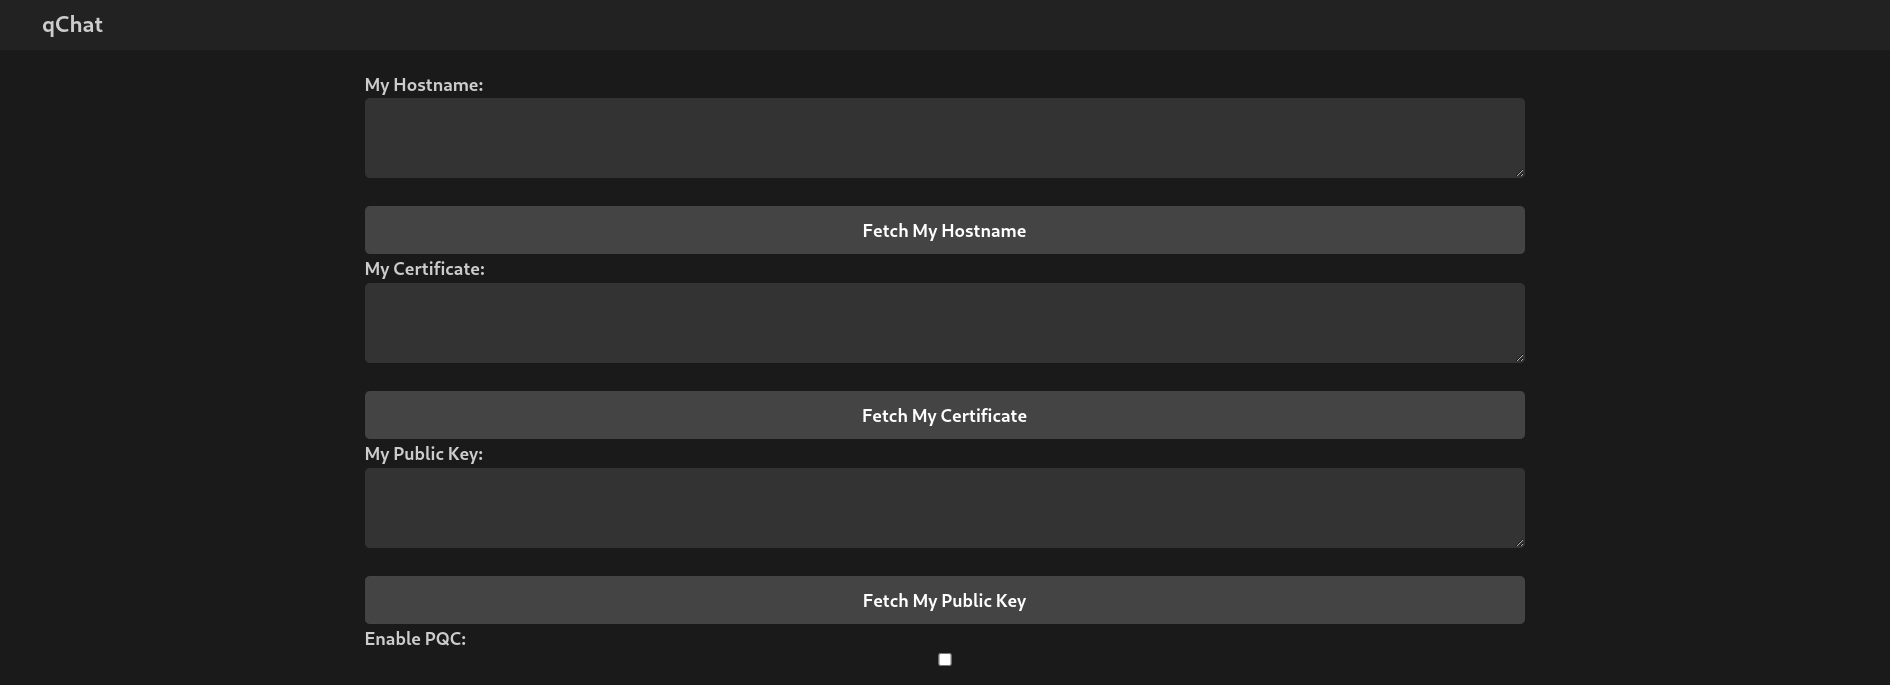
\includegraphics[width=1\linewidth]{resources/client/OwnUserCertKey.png}
    \caption{GUI: User}
    \label{fig:ownUser}
\end{figure}



\subsection{Registration Friends}

\textbf{Save Certificate:}\\
This feature allows users to add friends to their communication network. This involves entering the friend's onion address and certificate. Once both users have saved each other's onion address and certificate, they can begin communicating.\\

\textbf{Save PQC Public Key:}\\
For enhanced message security using PQC, users need to store the public key of the person they are communicating with. This creates a shared secret that allows both parties to encrypt messages using PQC. Importantly, once one user has saved the other's public key, both can communicate encrypted without the other user having to store a public key separately. This is due to the nature of the key exchange, which will be discuessed in \ref{sec:pqcworkflow}.

\begin{figure}[H]
    \centering
    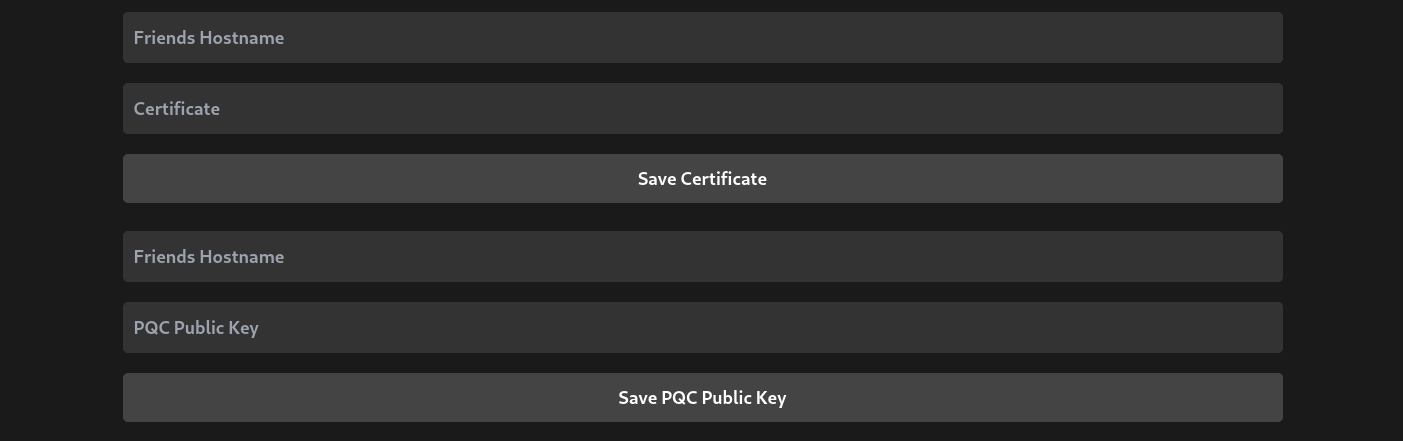
\includegraphics[width=1\linewidth]{resources/client/RegistrationFriend.png}
    \caption{GUI: Friend Registration}
    \label{fig:friendReg}
\end{figure}

\subsection{Send messages}
After this initial setup, the user can send text messages by selecting a recipient and composing the message.
Below is an example, of how such a chat could look like when fully configured (i.e. when Alice and Bob share there Onion Hostname, XMPP Certificate and (optionally) the PQC Public key.)
\begin{figure}[H]
    \centering
    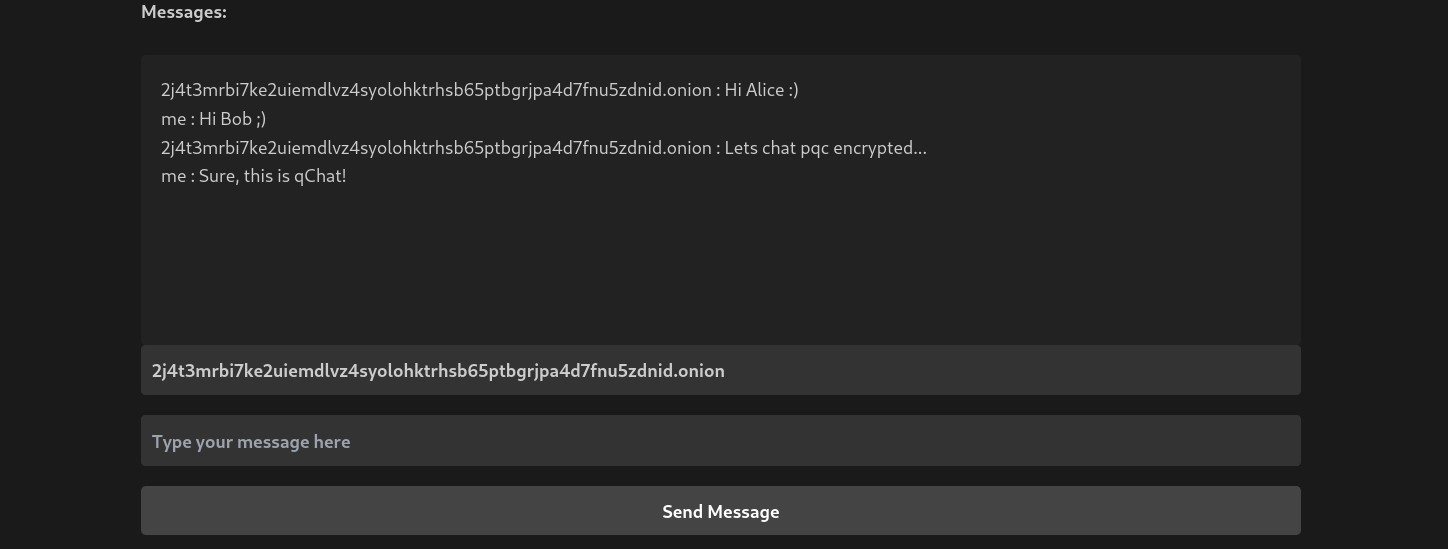
\includegraphics[width=1\linewidth]{resources/client/SendMessages.png}
    \caption{GUI: Send Messages}
    \label{fig:sendMessages}
\end{figure}
